\documentclass[a4paper,10pt]{article}

\usepackage[T1]{fontenc}
\usepackage[margin=0.72in]{geometry}
\usepackage{amsmath}
\usepackage{array}
\usepackage{booktabs}
\usepackage{csvsimple}
\usepackage{graphicx}
\usepackage{longtable}
\usepackage{microtype}
\usepackage{placeins}

% All displayed table rows are read from root-level CSV files.
\newcommand{\csvcomma}{,}
\newcommand{\csvrowstwo}[1]{%
  \csvreader[head to column names,late after line=\\]{#1}{}{\colA & \colB}}
\newcommand{\csvrowsfive}[1]{%
  \csvreader[head to column names,late after line=\\]{#1}{}{\colA & \colB & \colC & \colD & \colE}}
\newcommand{\csvrowssix}[1]{%
  \csvreader[head to column names,late after line=\\]{#1}{}{\colA & \colB & \colC & \colD & \colE & \colF}}
\newcommand{\csvrowsseven}[1]{%
  \csvreader[head to column names,late after line=\\]{#1}{}{\colA & \colB & \colC & \colD & \colE & \colF & \colG}}
\newcommand{\csvrowseight}[1]{%
  \csvreader[head to column names,late after line=\\]{#1}{}{\colA & \colB & \colC & \colD & \colE & \colF & \colG & \colH}}
\newcommand{\csvlongtable}[7]{%
  \begin{longtable}{#1}
  \caption{#2}\label{#3}\\
  \toprule
  #5 \\
  \midrule
  \endfirsthead
  \multicolumn{#4}{c}{\tablename\ \thetable\ continued}\\
  \toprule
  #5 \\
  \midrule
  \endhead
  \midrule\multicolumn{#4}{r}{Continued on next page}\\
  \endfoot
  \bottomrule
  \endlastfoot
  #7{#6}
  \end{longtable}%
}

\renewcommand{\thetable}{S\arabic{table}}
\renewcommand{\thefigure}{S\arabic{figure}}
\setlength\LTleft{0pt}
\setlength\LTright{0pt}

\title{Supplementary Material\\Enforcement of Mass Conservation and Non-Negativity in Statistical Surrogates of Activated Sludge Systems}
\author{}
\date{}

\begin{document}

\maketitle

\section{Scope and Reporting Convention}

This supplement reports detailed supporting results for the study. The benchmark contains 13 statistical surrogates, eleven nested in-distribution sample totals, five persistent outer folds, and two separately simulated out-of-distribution regimes. Raw and projected predictions always refer to the same observations. No out-of-distribution response entered fitting, preprocessing, hyperparameter selection, or normalization.

For component $j$, the reported component nRMSE is
\begin{equation}
\mathrm{nRMSE}_j=
\frac{\sqrt{n^{-1}\sum_{i=1}^{n}(\hat c_{ij}-c_{ij})^2}}
{\sigma_j^{(\mathcal T)}},
\end{equation}
where $\sigma_j^{(\mathcal T)}$ is the population SD of that component in the applicable training reference. For a derived composite $q\in\{\mathrm{COD},\mathrm{TN},\mathrm{TP},\mathrm{TSS}\}$, the requested composite-specific counterpart is
\begin{equation}
\mathrm{nRMSE}_q=
\frac{\sqrt{n^{-1}\sum_{i=1}^{n}(\hat y_{iq}-y_{iq})^2}}
{\sigma_q^{(\mathcal T)}}.
\end{equation}
The in-distribution denominator is estimated on the applicable outer-training partition; the out-of-distribution denominator is estimated once on all 10,000 in-distribution targets. Composite nRMSE is a secondary, composite-specific normalization and is not the primary nRMSE obtained by averaging squared standardized errors across all 20 effluent components.

In-distribution values are the arithmetic mean $\pm$ sample SD across five outer folds. Each $\Delta$ is calculated within a paired raw/projected fold before those five differences are summarized. Out-of-distribution values are single descriptive summaries over 600 cases and therefore have no fold SD. No hypothesis tests, confidence intervals, or inferential rank claims are reported.

\section{Benchmark Contract and Dataset Verification}

The 22 inputs were hydraulic retention time, aeration, and 20 influent concentrations. Each surrogate jointly or componentwise predicted the same 20 effluent concentrations in the fixed order $S_O$, $S_F$, $S_A$, $S_{NH4}$, $S_{NO2}$, $S_{NO3}$, $S_{N2}$, $S_{PO4}$, $S_I$, $S_{ALK}$, $X_I$, $X_S$, $X_H$, $X_{PAO}$, $X_{PP}$, $X_{PHA}$, $X_{AOB}$, $X_{NOB}$, $X_{MeP}$, and $X_{MeOH}$. COD, TN, TP, and TSS were calculated after prediction through the same fixed linear composition map for raw and projected outputs.

The surrogate roster comprised XGBoost, LightGBM, CatBoost, AdaBoost, Random Forest, Extra Trees, SVR, $k$-NN, PLS, Multi-task Elastic Net, Multi-task Lasso, MLP, and TabNet. PLS and the two multi-task linear surrogates form the prespecified Interpretable surrogates category because they expose one global coefficient structure; this label does not imply causal interpretation.

\begin{table}[htbp]
\centering
\caption{Mechanistic dataset generation and invariant verification. The invariant residual is $\|Ac_{out}-Ac_{in}\|_2$.}
\label{tab:s_dataset_validation}
\small
\begin{tabular}{lrrrrr}
\toprule
Dataset & Attempted & Retained & Acceptance (\%) & Maximum residual & Minimum component \\
\midrule
\csvrowssix{supp_table_s_dataset_validation.csv}
\bottomrule
\end{tabular}
\end{table}

The in-distribution accuracy summary contains $13\times11\times5\times2=1{,}430$ surrogate--size--fold--prediction rows. Component and composite summaries contain the corresponding 20-component and four-composite expansions. Tuning completed five 100-trial outer-fold studies and one separate 100-trial full-data study per surrogate, for 7,800 completed trials. The out-of-distribution benchmark used one full-data refit per surrogate and retained 600 mechanistic cases per regime.

\section{Detailed In-Distribution Predictive Performance}

Table~\ref{tab:s_id_component_accuracy} gives the same standardized error scale as the primary main-text metric at the individual-component level. The table contains all 260 surrogate--component combinations at $N=10{,}000$ and preserves raw/projected pairing. Projection lowered mean component nRMSE in 188 combinations (72.3\%) and for a majority of components in 12 of 13 surrogates; AdaBoost was the exception at 9 of 20.

\begingroup
\scriptsize
\setlength{\tabcolsep}{2.2pt}
\csvlongtable
  {llp{3.1cm}rrrrr}
  {Full-size in-distribution accuracy by effluent component and surrogate. Values are five-fold mean $\pm$ sample SD; $\Delta$ is projected minus raw on paired folds.}
  {tab:s_id_component_accuracy}
  {8}
  {Component & Unit & Surrogate & Raw nRMSE$_j$ & Projected nRMSE$_j$ & $\Delta$nRMSE$_j$ & Raw $R^2_j$ & Projected $R^2_j$}
  {supp_table_s_id_component_accuracy.csv}
  {\csvrowseight}
\endgroup

\clearpage
Table~\ref{tab:s_id_composite_accuracy} reports composite-normalized RMSE for COD, TN, TP, and TSS. Projection lowered TN and TP error for every surrogate but increased COD and TSS error for every surrogate.

\begingroup
\scriptsize
\setlength{\tabcolsep}{3pt}
\csvlongtable
  {lp{3.1cm}rrrrr}
  {Full-size in-distribution accuracy by derived water-quality composite and surrogate. Composite nRMSE is physical-unit RMSE divided by the population SD of that composite in the applicable outer-training partition. Values are five-fold mean $\pm$ sample SD and $\Delta$ is projected minus raw on paired folds.}
  {tab:s_id_composite_accuracy}
  {7}
  {Composite & Surrogate & Raw nRMSE$_q$ & Projected nRMSE$_q$ & $\Delta$nRMSE$_q$ & Raw $R^2$ & Projected $R^2$}
  {supp_table_s_id_composite_accuracy.csv}
  {\csvrowsseven}
\endgroup

\section{Mass-Conservation, Non-Negativity, and Positivity Backtracking}

All 750,750 raw in-distribution predictions violated the declared mass-conservation tolerance. Raw non-negativity violations varied by surrogate and sample size. After projection, every in-distribution prediction satisfied mass conservation within tolerance and contained no negative concentration; the maximum projected conservation residual was $2.06\times10^{-13}$.

Positivity backtracking was activated for 2,489 predictions (0.332\%). Random Forest, PLS, and Extra Trees accounted for 2,044 activations (82.1\%) and had among the largest standardized projection displacements. Table~\ref{tab:s_backtracking} distinguishes the cumulative count from the activation rate so that the larger number of evaluated rows at high sample totals is not mistaken for a rising backtracking propensity.

\begingroup
\small
\setlength{\tabcolsep}{4pt}
\csvlongtable
  {lrrrr}
  {Positivity-backtracking activation by surrogate. The all-size denominator is 57,750 projections per surrogate; the final two columns describe $N=10{,}000$.}
  {tab:s_backtracking}
  {5}
  {Surrogate & All-size count & All-size rate (\%) & Full-size rate (\%) & Full-size mean $d_c^{\mathrm{std}}$}
  {supp_table_s_backtracking.csv}
  {\csvrowsfive}
\endgroup

\section{Computational Performance}

Fit time includes fold-local preprocessing and surrogate fitting, but excludes Optuna search, model saving, prediction, and projection. Inference timing used a deterministic 512-row batch, five warm-up calls, and 30 measured calls. Values in Table~\ref{tab:s_timing} are five-fold mean $\pm$ sample SD. Search duration is omitted because each fold-specific study was reused at all eleven nested sizes and therefore is not a size-specific training cost.

Training-time scaling differed much more strongly than inference latency (Figure~\ref{fig:s_training_time_scaling}). At $N=10{,}000$, mean fold-local preprocessing and fitting time ranged from 0.024 s for Multi-task Elastic Net to 56.0 s for SVR. Multi-task Lasso and $k$-NN also fitted in approximately 0.03 s, whereas MLP and TabNet required 20.5 and 24.7 s, CatBoost 33.3 s, and SVR 56.0 s. SVR showed the steepest growth, from 0.054 s at $N=500$ to 56.0 s at $N=10{,}000$, consistent with the scaling of kernel fitting. CatBoost remained near 31--33 s because its selected boosting work and fixed overhead dominated the change in row count. These fit times exclude the separate 100-trial hyperparameter searches and saving of fitted surrogates; they therefore describe refitting cost once settings have been selected. Complete values are reported in Table~\ref{tab:s_timing}.

The timing results sharpen the accuracy findings. MLP delivered the best full-size accuracy with moderate fitting time, while CatBoost and SVR were slower to refit under the selected settings. The multi-task linear surrogates were extremely fast and benefited from projection, but their final nRMSE remained higher than the nonlinear alternatives. Thus, projection does not remove the need to choose a surrogate appropriate to the desired accuracy--training-cost tradeoff; it adds a common feasibility layer after that choice has been made.

\begin{figure}[htbp]
\centering
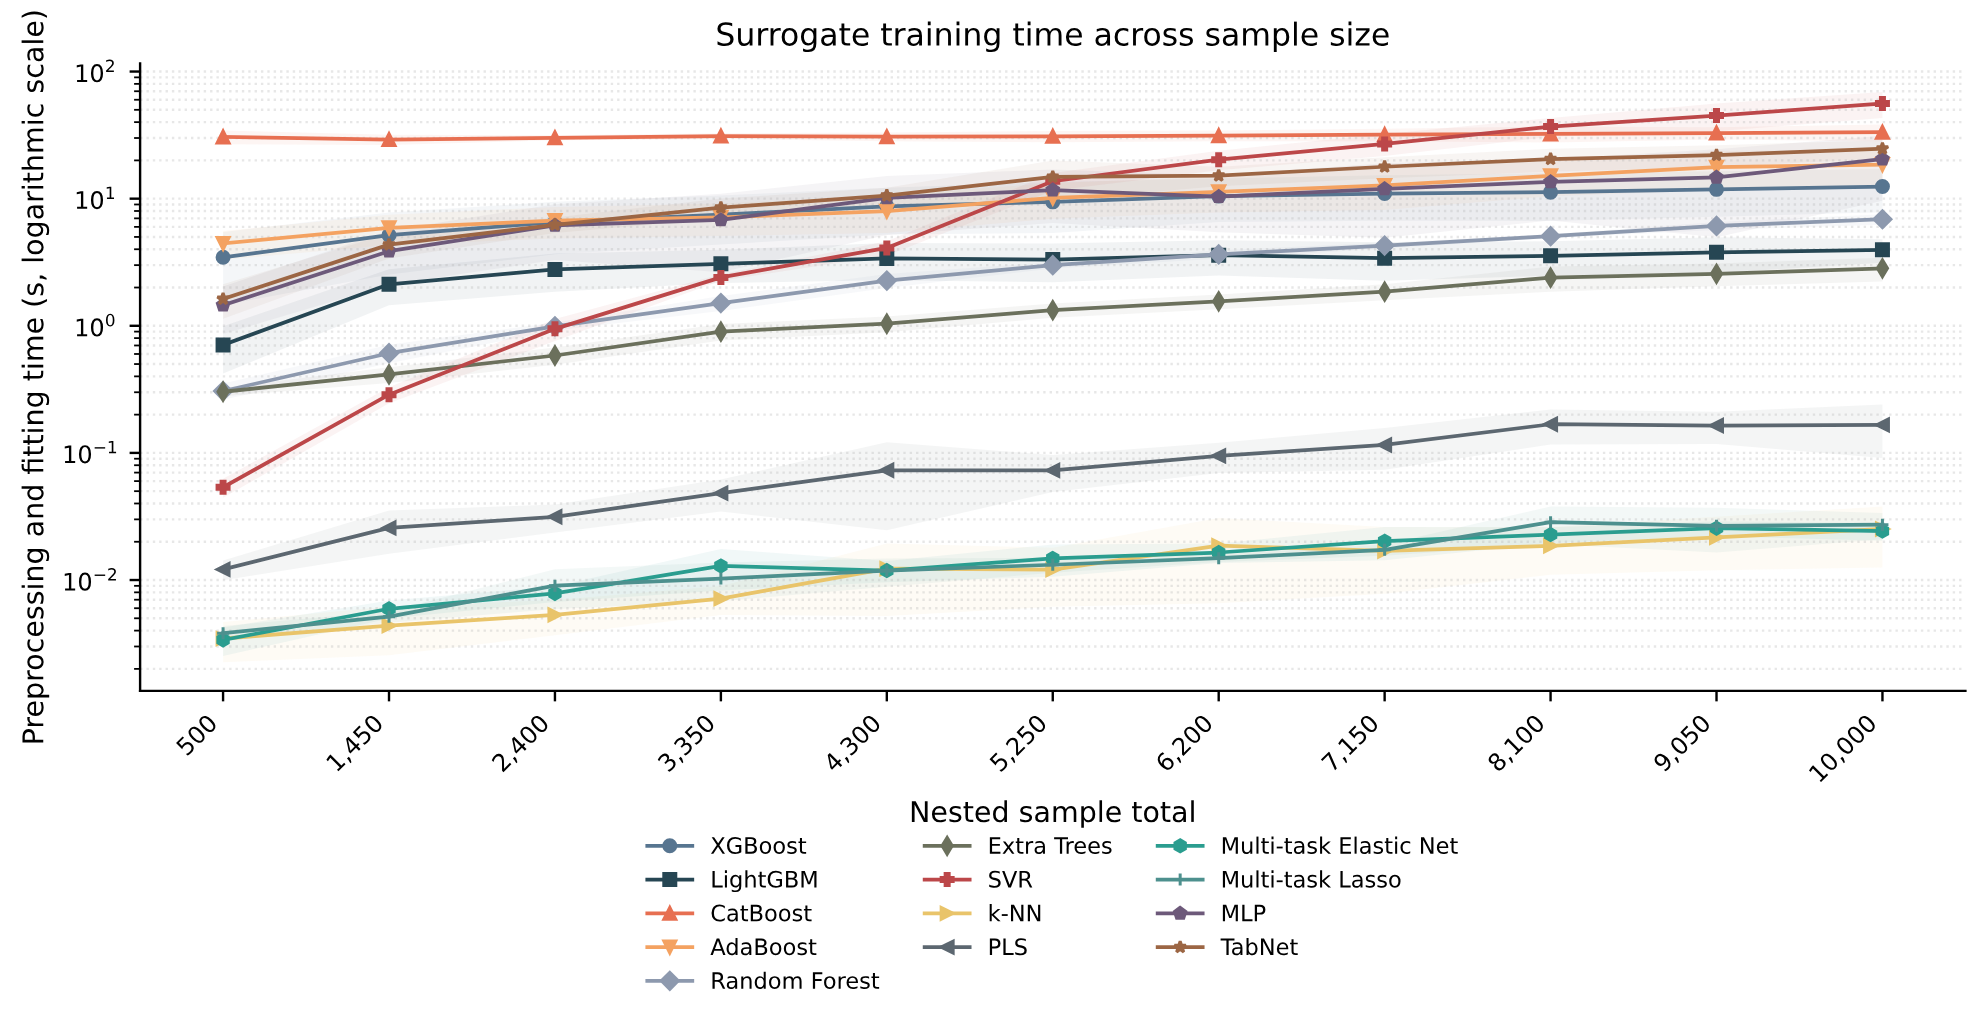
\includegraphics[width=0.96\textwidth]{supp_figure_training_time_scaling.png}
\caption{In-distribution preprocessing and surrogate-fitting time across nested sample totals. Lines show five-fold means, shaded regions show $\pm$ one sample SD, and the vertical axis is logarithmic. Hyperparameter-search time is excluded.}
\label{fig:s_training_time_scaling}
\end{figure}

At $N=10{,}000$, complete 20-component raw inference ranged from approximately 0.001 ms per sample for PLS and the multi-task linear surrogates to 1.874 ms per sample for SVR (Figure~\ref{fig:s_inference_latency}). Projection-only latency ranged from 0.068 to 0.144 ms per sample across surrogates. The projection therefore dominated end-to-end latency for the fastest linear predictors but remained below 0.15 ms per sample under the stated batching protocol. All 766,350 production projections used the QR solver; the SVD fallback was not activated. Consequently, projection supplied deterministic mass-conservation and non-negativity enforcement at a small absolute deployment cost. This makes the method especially attractive for downstream screening, optimization, or decision-support loops in which infeasible concentration vectors are more damaging than a sub-millisecond correction step.

\begin{figure}[htbp]
\centering
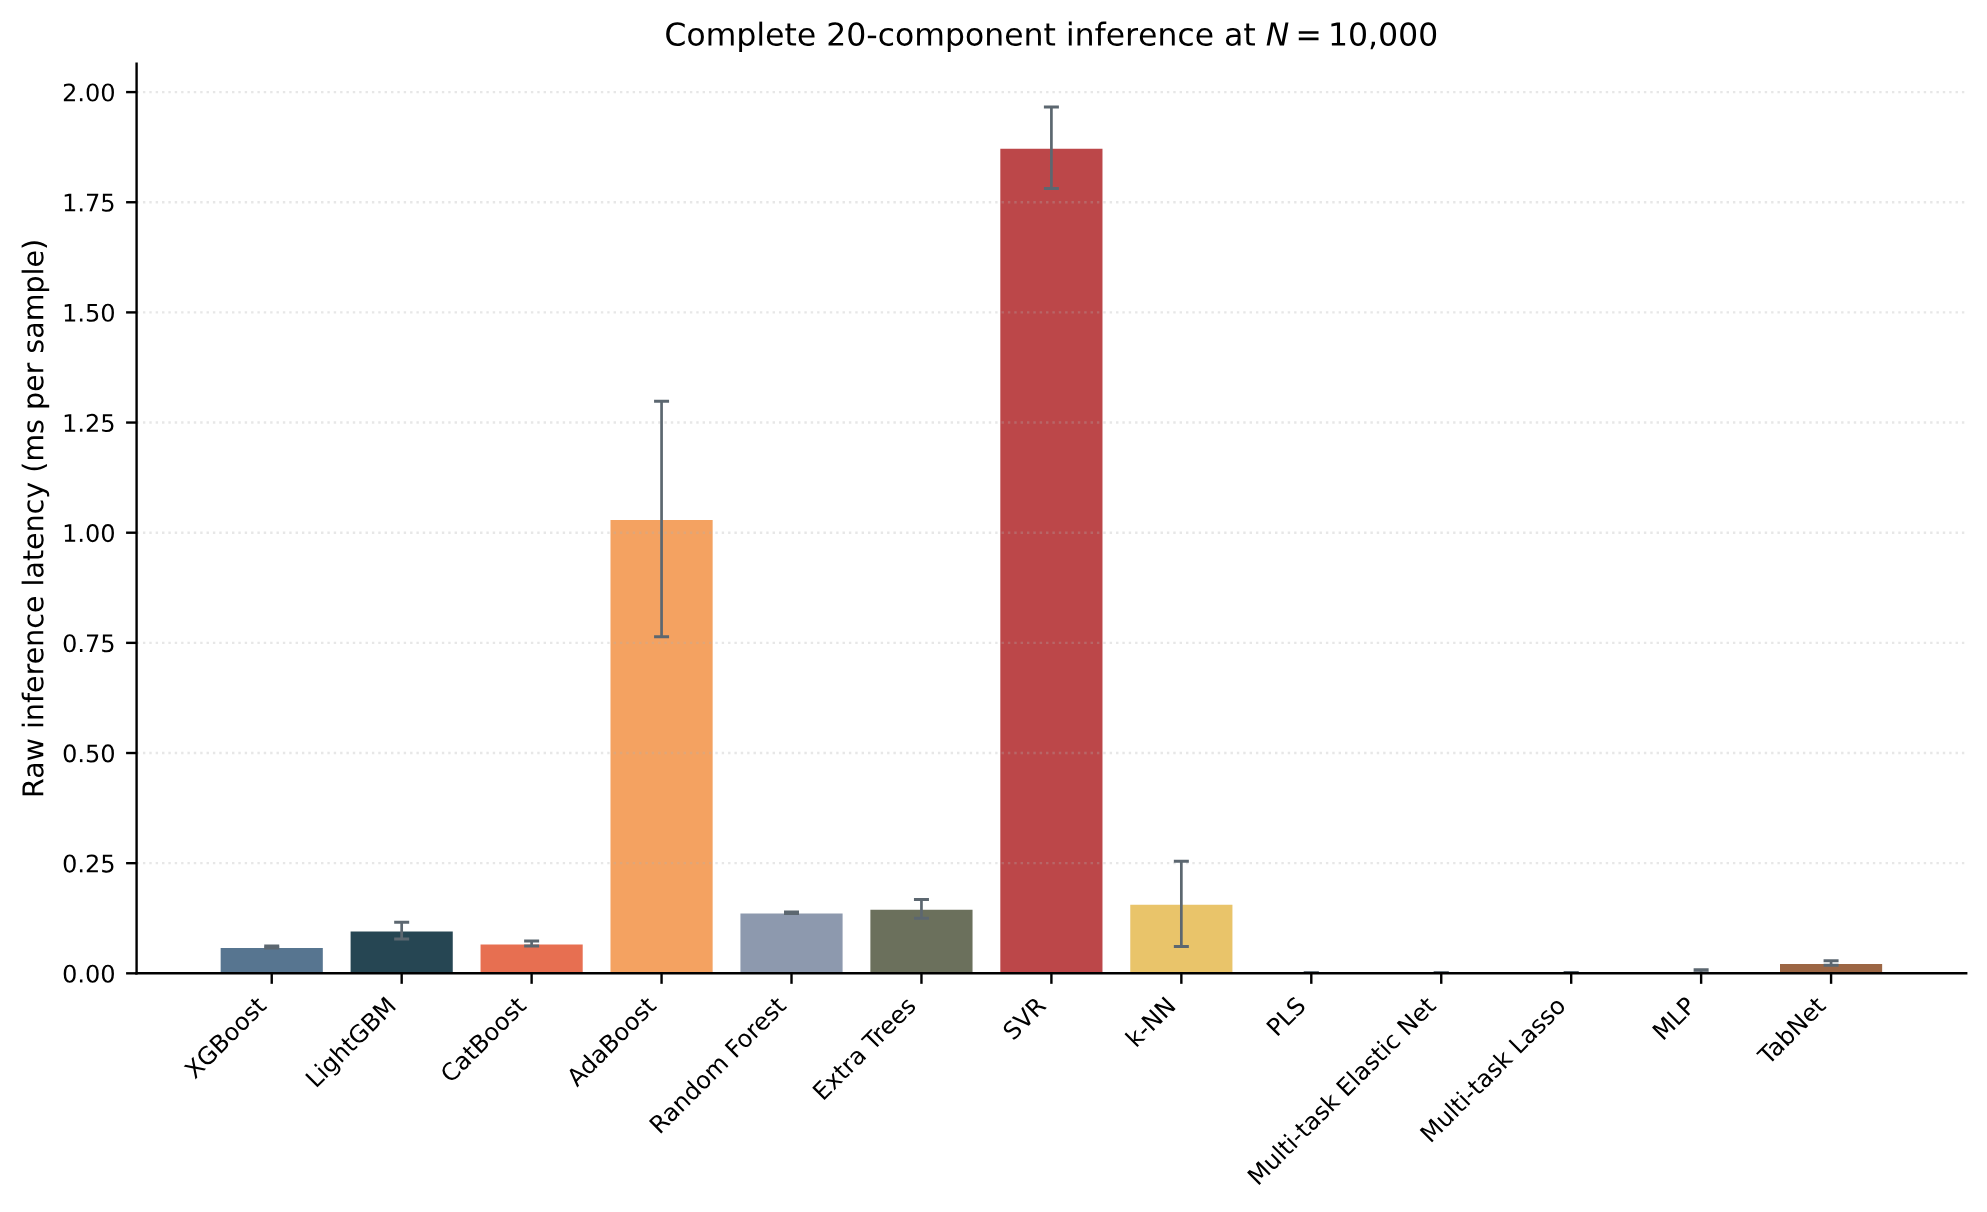
\includegraphics[width=0.94\textwidth]{supp_figure_inference_latency.png}
\caption{Complete 20-component raw surrogate-inference latency at $N=10{,}000$. Bars show the five-fold mean and error bars show $\pm$ one sample SD of fold medians.}
\label{fig:s_inference_latency}
\end{figure}

\FloatBarrier

\begingroup
\small
\setlength{\tabcolsep}{3.5pt}
\csvlongtable
  {lrrrrr}
  {Computational timing summary. Fit time includes fold-local preprocessing and surrogate fitting but excludes hyperparameter search; latency is milliseconds per sample. Values are five-fold mean $\pm$ sample SD.}
  {tab:s_timing}
  {6}
  {Surrogate & Fit at $N=500$ (s) & Fit at $N=10{,}000$ (s) & Fit-time ratio & Raw latency & Projection latency}
  {supp_table_s_timing.csv}
  {\csvrowssix}
\endgroup

\section{Detailed Out-of-Distribution Results}

The mild and severe out-of-distribution tables use the same 600 cases before and after projection. Component nRMSE uses the fixed full in-distribution component SD, and composite nRMSE uses the corresponding full in-distribution composite SD. Projection lowered aggregate 20-component nRMSE for 11 of 13 surrogates under mild extrapolation and 9 of 13 under severe extrapolation. At component level, it lowered 192 of 260 mild comparisons (73.8\%) and 193 of 260 severe comparisons (74.2\%).

\subsection{Mild Extrapolation}

\begingroup
\scriptsize
\setlength{\tabcolsep}{2.2pt}
\csvlongtable
  {llp{3.1cm}rrrrr}
  {Mild out-of-distribution accuracy by effluent component and surrogate. Each value summarizes the same 600 mechanistic cases; $\Delta$ is projected minus raw.}
  {tab:s_ood_mild_component_accuracy}
  {8}
  {Component & Unit & Surrogate & Raw nRMSE$_j$ & Projected nRMSE$_j$ & $\Delta$nRMSE$_j$ & Raw $R^2_j$ & Projected $R^2_j$}
  {supp_table_s_ood_mild_component_accuracy.csv}
  {\csvrowseight}
\endgroup

\clearpage
\begingroup
\scriptsize
\setlength{\tabcolsep}{3pt}
\csvlongtable
  {lp{3.1cm}rrrrr}
  {Mild out-of-distribution accuracy by derived water-quality composite and surrogate. Composite nRMSE is physical-unit RMSE divided by the population SD of that composite in all 10,000 in-distribution targets. Each value summarizes the same 600 mechanistic cases; $\Delta$ is projected minus raw.}
  {tab:s_ood_mild_composite_accuracy}
  {7}
  {Composite & Surrogate & Raw nRMSE$_q$ & Projected nRMSE$_q$ & $\Delta$nRMSE$_q$ & Raw $R^2$ & Projected $R^2$}
  {supp_table_s_ood_mild_composite_accuracy.csv}
  {\csvrowsseven}
\endgroup

\subsection{Severe Extrapolation}

\begingroup
\scriptsize
\setlength{\tabcolsep}{2.2pt}
\csvlongtable
  {llp{3.1cm}rrrrr}
  {Severe out-of-distribution accuracy by effluent component and surrogate. Each value summarizes the same 600 mechanistic cases; $\Delta$ is projected minus raw.}
  {tab:s_ood_severe_component_accuracy}
  {8}
  {Component & Unit & Surrogate & Raw nRMSE$_j$ & Projected nRMSE$_j$ & $\Delta$nRMSE$_j$ & Raw $R^2_j$ & Projected $R^2_j$}
  {supp_table_s_ood_severe_component_accuracy.csv}
  {\csvrowseight}
\endgroup

\clearpage
\begingroup
\scriptsize
\setlength{\tabcolsep}{3pt}
\csvlongtable
  {lp{3.1cm}rrrrr}
  {Severe out-of-distribution accuracy by derived water-quality composite and surrogate. Composite nRMSE is physical-unit RMSE divided by the population SD of that composite in all 10,000 in-distribution targets. Each value summarizes the same 600 mechanistic cases; $\Delta$ is projected minus raw.}
  {tab:s_ood_severe_composite_accuracy}
  {7}
  {Composite & Surrogate & Raw nRMSE$_q$ & Projected nRMSE$_q$ & $\Delta$nRMSE$_q$ & Raw $R^2$ & Projected $R^2$}
  {supp_table_s_ood_severe_composite_accuracy.csv}
  {\csvrowsseven}
\endgroup

Every raw out-of-distribution prediction set violated mass conservation. Projection eliminated mass-conservation and non-negativity violations across all 15,600 out-of-distribution surrogate predictions, with maximum projected conservation residual $1.72\times10^{-13}$. Positivity backtracking was activated 29 times under mild and 39 times under severe extrapolation.

\section{Full-Data Hyperparameters}

Table~\ref{tab:s_full_hyperparameters} records the selected settings used for the final full in-distribution refits and out-of-distribution evaluation. These settings were selected in separate four-fold, 100-trial studies using only in-distribution data.

\begingroup
\scriptsize
\setlength{\tabcolsep}{4pt}
\csvlongtable
  {p{3.2cm}p{11.5cm}}
  {Selected settings for the final full-data surrogate refits used in out-of-distribution evaluation. Fixed implementation controls are included because they form part of the specified fitting protocol.}
  {tab:s_full_hyperparameters}
  {2}
  {Surrogate & Selected full-data settings}
  {supp_table_s_full_hyperparameters.csv}
  {\csvrowstwo}
\endgroup

\end{document}
